\documentclass[journal]{IEEEtran}
\usepackage[utf8]{inputenc}
\ifCLASSINFOpdf
\else
\fi
\hyphenation{op-tical net-works semi-conduc-tor}
\usepackage{cite}
\usepackage{graphicx}
\usepackage[justification=centering]{caption}

\begin{document}
\title{Representación del Sistema Solar en OpenGL}

\author{Sebastián Lastra Mena, Amaro Escobar\\ \{sebastian.lastra@usach.cl\}, \{amaro.escobar@usach.cl\}\\Departamento de Matemáticas y Ciencia de la Computación \\ Universidad de Santiago de Chile - Avenida Libertador General Bernardo O'Higgins \#3363 
}

\markboth{TRABAJO DE INVESTIGACIÓN E IMPLEMENTACIÓN - CURSO DE COMPUTACIÓN GRÁFICA, Semestre II - Año 2014}
{Shell \MakeLowercase{\textit{et al.}}}

\maketitle

\begin{abstract}
	En este trabajo se presenta el modelamiento del sistema solar con cinturón de asteroides y la enana roja 	Némesis. Se creó en un ambiente gráfico el cual sufrirá los cambios dependiendo de la elipse que se establezca para la enana roja. Otras implementaciones realizadas en este trabajo fueron la aplicación de texturas en el fondo de la escena utilizando la técnica de SkyBox, el posicionamiento de la ViewPort en la orbita del planeta que se requiera y la implementación de un menu para facilitar la navegación entre las funcionalidades del programa. Fue implementado en OpenGL bajo sistema operativo GNU/Linux.
\end{abstract}

\begin{keywords}
	Sistema Solar, OpenGL, Orbita Elíptica, Nube de Oort, Némesis, SkyBox.
\end{keywords}

\IEEEpeerreviewmaketitle

\section{Introducción}

	La idea principal es llevar a cabo la simulación del Sistema Solar el cual incluye un cinturón de asteroides y la presencia de una enana roja. El sistema que simula el fenómeno espacial se activa presionando un botón, lo cual genera una onda expansiva que desplaza a los asteroides de su cinturón haciendo posible la colisión de estos con los distintos planetas del sistema solar.

	Considerando que lo que se presenta en esta versión del informe es una modificación a lo que ya está implementado, resulta importante mencionar que, pese a que se puede pensar que resulta más rápido, fácil e intuitivo implementar los nuevos requerimientos, se tomó gran parte del tiempo para leer, comprender, analizar e interactuar con el programa, con el fin de poder acoplar los nuevos requerimientos y no estropear el resto.

\subsection{Objetivo General}
	Generar gráficamente el modelamiento del fenómeno espacial y que se aprecie lo más realista posible. 

\subsection{Objetivos Específicos}
	\begin{itemize}
		\item Aprender a usar las herramientas necesarias de OpenGL para la realización de sombras, iluminación 
		y texturas.
		\item Entender los conceptos fundamentales de la Computación Gráfica y cómo se expresan y/o representan 
		en términos computacionales.
		\item Asociar la teoría aprendida en el curso de Computación Gráfica con la 
		representación práctica en OpenGL.
		\item Lograr un dominio en el lenguaje  de programación y librerías utilizadas.	
	\end{itemize}
	
\section{Definición de la problemática}

En el año 1984, surge una hipótesis astronómica que sustenta de que nuestro Sol forme parte de un sistema binario \cite{RAMuller}. En este sistema, la estrella compañera del sol se llamaría Némesis y cada 26 millones de años desestabiliza la nube de Oort, la cual posee gran cantidad de cometas y estrellas \cite{astronomia}. Esta desestabilización generaría que los cometas que se encuentran en la nube se dirijan hacia el sistema solar causando gran cantidad de colisiones en los planetas.

\subsection{Problemática}
Algunas de las problemáticas de nuestro modelamiento son:\\

\begin{enumerate}
	\item Calcular la trayectoria de los asteroides encontrados en la nube de Oort que impactarán con los planetas.
	\item Encontrar los planetas con los cuales efectivamente harán colisión.
	\item Correcta implementación de la nube de Oort, buscando la mejor representación utilizando OpenGL.
	\item Implementar un menú que permita navegar entre las distintas funcionalidades presentes en el programa.
	\item Aplicar la técnica de SkyBox en la escena.
	\item Realizar la traslación de la ViewPort hacía el planeta deseado utilizando el menú.
\end{enumerate}

\section{Modelo matemático}

\subsection{Ecuación de la elipse}

\begin{figure}[h!]
	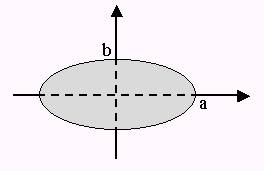
\includegraphics[width=0.25\textwidth, height=0.25\textwidth]{elipse.png}
	\centering
	\caption{Elipse}
\end{figure}

\newpage

\[ \scalebox{2}{$\frac{x^{2}}{a^{2}} + \frac{y^{2}}{b^{2}}$} \]\\

Donde $a>0$ y $b>0$, son las coordenadas de las abscisas. La elipse se encuentra centrada en el origen ($h,k=0$) \cite{enciclopedia}. La ecuación de la elipse modela la ubicación de la nube de Oort y la órbita de los planetas. Además, la trayectoria de la enana roja Némesis.\\

\[ \scalebox{2}{$ \frac{x\cdot(x-x_{0})}{a^{2}} + \frac{y\cdot(y-y_{0})}{b^{2}}$} \]\\

Luego, con la ecuación de la tangente a una elipse, se obtiene la dirección a la cual serán lanzadas las estrellas de la nube de Oort, y se observar las colisiones con los planetas del sistema solar.

\section{Aproximación utilizada en las simulaciones gráficas}

La formulación del modelo en base al sistema solar y a la teoría de la enana roja respecto al diagrama de Hertzsprung-Russell \cite{russel}, esto es un modelo debido a que los cálculos realizados son a escala respecto al sistema solar real, es decir, X pixeles son equivalentes a algunos años luz. Los tamaños de los planetas también son a escala y la formulación de las estrellas son pixeles arbitrarios dentro de un rango (cinturón de asteroides).

\section{Implementación computacional}

OpenGl es el principal entorno de desarrollo, para la creación de aplicaciones graficas portátiles e interactivas en  2D y 3D. Desde su introducción en 1992, OpenGl se ha convertido en la Interfaz de Programación de Aplicaciones (API) graficas más usada por la industria, brindando miles de aplicaciones a una gran variedad de plataformas de computación. A su vez, OpenGL fomenta la innovación y velocidad del desarrollo de aplicaciones incorporando una alta variedad de formas de rendering, mapeo de texturas, efectos especiales y otras poderosas funciones de visualización \cite{opengl}.\\

Se utilizo el Entorno de Desarrollo Integrado (IDE) llamado NetBeans, el cual permite detectar rápidamente errores de sintáxis. Permite también iniciar en modo debug, herramienta con la cual es posible realizar un seguimiento del valor de cada variable en cada frame de la aplicación. Además, resulta mucho más fácil el proceso de compilación. La instalación y posterior configuración del proyecto se escapan del ámbito de este informe pero se puede encontrar información respecto a esto en nuestra Wiki del proyecto en GitHub \cite{wiki}.\\

Finalmente, pese a que existe una gran variedad de librerías diferentes a OpenGL, no se utilizaron pues la idea principal de este proyecto es aprender a utilizar al más bajo nivel posible cada uno de los elementos presentes en la computación gráfica (Transformaciones geométricas, primitivas, etc...), cosa que es posible directamente con OpenGL y no con librerías externas que agregan una capa de abstracción en la programación y, por lo tanto, un menor nivel de entendimiento de lo que se realiza. Además, la mayoría de dichas librerías sólo están disponibles para C++.

\section{Análisis de resultados}

\subsection{Validación de resultados}

 El trabajo es realizado es en base a un proyecto anterior del ramo de Computación Gráfica, llamado Sistema Solar (5). Este proyecto ha sido optimizado en líneas de código y utilizado para nuestro proyecto de fin de semestre. El hecho de que la nube de Oort no se pueda apreciar desde nuestro planeta, y de que la estrella Némesis sea una hipótesis astronómica, deja a la “realidad” un poco de lado. Se corresponde sí a las hipótesis científicas, a las distancias normalizadas de los planetas y sus velocidades de rotación.

\subsection{Rendimiento gráfico de la aplicación}

La aplicación realizada quedo implementada de tal manera que su visualización es, si no rápida, realista a un nivel a escala del fenómeno real es decir, podría verse tanto en un pc especializado (poseedor de una buena tarjeta de video) o en un pc común  corriente. La aplicación es optima respecto al trabajo que tomamos de base, ya que se redujeron las líneas de código, sin perder la efectividad y el fondo de la aplicación destacando estos 2 puntos anteriores, creemos que el rendimiento grafico de la aplicación es prudente(por la sencillez), rápido(por como se aprecia) y optimo(por cómo se realiza).

\subsection{Resultados y Problemáticas}

Como problema de implementación, tenemos un equipo al cual se le instaló el SO Linux Ubuntu, el cual no posee aceleración gráfica, por lo que el proyecto no alcanza su apogeo corriendo en esa máquina. No se alcanza a distinguir los movimientos de los planetas y pierde valores al momento de compilar. Por ende, la programación en ese equipo se ha vuelto truncado por problemas que escapan a cualquier tipo de solución que podamos dar. 

\section{Experimentos}

En la figura 1 se puede apreciar la estrella Némesis (situada en la esquina inferior derecha) sin haber tocado los asteroides de la nube de Oort. Posteriormente en la figura 2 se puede ver como son desplazados los asteroides al perder su órbita normal y ser atraídos por el sol.

\section{Conclusiones}

La realización de este modelamiento fue costosa y ardua, ya que no había conocimiento de cómo plantearnos el problema, tal vez bosquejos o ideas que cualquier persona podría tener, pero no como analistas. Luego de algunas clases y laboratorios empezamos a entender lo que nos pedían y como poder realizar el modelamiento. Después de mucha investigación, comprensión de códigos antiguos, adquisición de conocimientos sobre el lenguaje de programación utilizado y el trabajo de unas funciones, se pudo llevar a cabo el modelamiento final. Nos sentimos orgullosos de haber sido capaces de realizar un buen modelamiento de un fenómeno natural tan sorprendente. De aquí en adelante esperamos que este trabajo pueda ser reutilizado como base para proyectos mas grandes por alumnos que tendrán este ramo más adelante o bien ser capaz de optimizarlo y lograr difundirlo para algún uso particular de buena manera.

\bibliographystyle{IEEEtran}
\bibliography{bibi}

\end{document}